\documentclass[9pt]{innovativeinnovation-cheatsheet}

\cheatsheettitle{\ding{93} Snowflake logs ingestion and querying cheatsheet \ding{93}}

\begin{document}
\begin{multicols}{3}

\cheatsheetsection{Snowflake SQL basics}

\cheatsheetsubsection{Useful links}
\be{}
      \item \href{https://app.snowflake.com/}{New Web GUI}
      \item \href{https://docs.snowflake.com/en/sql-reference-commands.html}{Snowflake SQL reference}
\ee{}

\cheatsheetsection{Sample data}
\newline
Logs table structure
\scriptsize	
\\[4pt]
\begin{tabular}{| m{16em} | m{10em}| m{10em} |}
      \hline
      \texttt{DATA} & \texttt{EVENT\_TIME} & \texttt{PARSE\_TIME}\\
      \hline
      \texttt{\{"user":"testuser","category"..} & \texttt{2022-04-25T10:04:03Z} & \texttt{2022-04-25T10:09:55Z}\\
      \hline
\end{tabular}

\small
\noindent Data field content
\scriptsize		
\\[-18pt]
\begin{lstlisting}[style=code_style]
{
      "user": "testuser",
      "category": "login",
      "cloud": "AWS",
      "time": "2022-04-25T10:04:03Z",
      "result": "success",
      "ip_address": "10.0.0.1"
}
\end{lstlisting}

%%%%%%%%%%% Querying single table
\cheatsheetsection{Querying single table}
\cheatsheetsubsection{Describe}
\small
Describes the structure of the requested item (database, table, etc).
\\[-18pt]
\begin{lstlisting}[style=code_style]
describe table DB_NAME.SCHEMA_NAME.TABLE_NAME;
\end{lstlisting}
Output:
\\[-18pt]
\begin{lstlisting}[style=code_style]
name        type              kind
DATA        VARIANT           COLUMN
EVENT_TIME  TIMESTAMP_NTZ(9)  COLUMN
PARSE_TIME  TIMESTAMP_NTZ(9)  COLUMN
\end{lstlisting}
\small
Fetch all columns from the log table:
\\[-18pt]
\begin{lstlisting}[style=code_style]
SELECT *
FROM RAW_LOG_TABLE;
\end{lstlisting}
\small
Fetch \texttt{DATA} column from the log table:
\\[-18pt]
\begin{lstlisting}[style=code_style]
SELECT DATA
FROM RAW_LOG_TABLE;
\end{lstlisting}
\small
Fetch \texttt{DATA} sorted by the \texttt{EVENT\_TIME} column in the default ASCending order
\\[-18pt]
\begin{lstlisting}[style=code_style]
SELECT DATA
FROM RAW_LOG_TABLE
ORDER BY EVENT_TIME ASC;
\end{lstlisting}
\small
Fetch \texttt{DATA} sorted by the \texttt{EVENT\_TIME} column in the default DESCending order
\\[-18pt]
\begin{lstlisting}[style=code_style]
SELECT DATA
FROM RAW_LOG_TABLE
ORDER BY EVENT_TIME DESC;
\end{lstlisting}
\small
Fetch subkey \texttt{ip\_address} from \texttt{DATA} sorted by the \texttt{EVENT\_TIME} column in the default DESCending order
\\[-18pt]
\begin{lstlisting}[style=code_style]
SELECT DATA:ip_address
FROM RAW_LOG_TABLE
ORDER BY EVENT_TIME DESC;
\end{lstlisting}

%%%%%%%%%% Limit/order
\cheatsheetsubsection{Limit/Order}
\small
\vspace{-18pt}
\bi{}
\item \texttt{ORDER BY} for \textbf{large result sets should be used with filtering}, as the command requires to fetch the matching results first to perform the order operation
\item \texttt{TOP <n>} and \texttt{LIMIT <count>} are equivalent (can be used interchangeably)
\item \texttt{LIMIT <count> [ OFFSET <start> ]}\newline can be used interchangeably to:\newline \texttt{[ OFFSET <start> ] [ { ROW | ROWS } ] FETCH [ { FIRST | NEXT } ] <count> [ { ROW | ROWS } ] [ ONLY ]}
\ei{}
Following queries are equivalent:
\scriptsize
\\[-18pt]
\begin{lstlisting}[style=code_style]
SELECT DATA:ip_address as ip_address
FROM RAW_LOG_TABLE
ORDER BY EVENT_TIME
LIMIT 100;

SELECT TOP 100 DATA:ip_address as ip_address
FROM RAW_LOG_TABLE
ORDER BY EVENT_TIME;

SELECT DATA:ip_address as ip_address
FROM RAW_LOG_TABLE
ORDER BY EVENT_TIME
FETCH FIRST 100;
\end{lstlisting}

%%%%%%%%%% Aliases
\cheatsheetsubsection{Aliases}
\small
Columns
\\[-18pt]
\begin{lstlisting}[style=code_style]
SELECT DATA:ip_address as ip_address
FROM RAW_LOG_TABLE;
\end{lstlisting}
\small
Tables
\\[-18pt]
\begin{lstlisting}[style=code_style]
SELECT DATA:ip_address
FROM RAW_LOG_TABLE as logs;
\end{lstlisting}

%%%%%%%%%% Timestamps
\cheatsheetsubsection{Timestamps}
\vspace{-18pt}
\bi{}
\item \texttt{TIMESTAMP\_TZ} \ding{239} timestamp with time zone, converting function: \texttt{TO\_TIMESTAMP\_TZ(string)}
\item \texttt{TIMESTAMP\_LTZ} \ding{239} timestamp with local time zone, converting function: \texttt{TO\_TIMESTAMP\_LTZ(string)}
\item \texttt{TTIMESTAMP\_NTZ} \ding{239} timestamp with no time zone, converting function: \texttt{TO\_TIMESTAMP\_NTZ(string)})
\ei{}

\small
Time conversion by function
\\[-18pt]
\begin{lstlisting}[style=code_style]
SELECT TO_TIMESTAMP_NTZ('2013-04-05 01:02:03');
\end{lstlisting}
\small
Time conversion by cast operation
\\[-18pt]
\begin{lstlisting}[style=code_style]
SELECT '2013-04-05 01:02:03'::TIMESTAMP_NTZ
\end{lstlisting}

%%%%%%%%%% Timestamps
\cheatsheetsubsection{Time operations}
Get current timestamp
\\[-18pt]
\begin{lstlisting}[style=code_style]
SELECT CURRENT_TIMESTAMP();
\end{lstlisting}
Add the specified value for the specified date or time
\\[-18pt]
\begin{lstlisting}[style=code_style]
SELECT DATEADD(day, -1, current_timestamp());
\end{lstlisting}
Calculate the difference between two date
\\[-18pt]
\begin{lstlisting}[style=code_style]
SELECT DATEDIFF(day, '2021-01-01'::date, '2021-02-28'::date)
\end{lstlisting}

%%%%%%%%%% Filtering the output
\cheatsheetsubsection{Filtering the output}
Compare
\\[-18pt]
\begin{lstlisting}[style=code_style]
SELECT DATA:user
FROM
WHERE EVENT_TIME > DATEADD(day, -1, current_timestamp());
\end{lstlisting}
Between
\\[-18pt]
\begin{lstlisting}[style=code_style]
SELECT DATA:user
FROM
WHERE EVENT_TIME BETWEEN DATEADD(day, -2, current_timestamp())
      AND DATEADD(day, -1, current_timestamp())
\end{lstlisting}

Not equal
\\[-18pt]
\begin{lstlisting}[style=code_style]
SELECT DATA
FROM
WHERE DATA:ip_address != '1.1.1.1';
\end{lstlisting}

Equal
\\[-18pt]
\begin{lstlisting}[style=code_style]
SELECT DATA
FROM
WHERE DATA:result = 'success';
\end{lstlisting}

Not null
\\[-18pt]
\begin{lstlisting}[style=code_style]
SELECT DATA
FROM
WHERE DATA:result IS NOT NULL;
\end{lstlisting}

In
\\[-18pt]
\begin{lstlisting}[style=code_style]
SELECT DATA
FROM
WHERE DATA:result IN ('success', 'failure');
\end{lstlisting}

%%%%%%%%%% Refering to previous results
\cheatsheetsubsection{Refering to previous queries and results}
\vspace{-18pt}
\be{}
\item Snowflake stores all query results for 24 hours.
\item Result sets do not have any metadata associated with them, so processing large results might be slower than if you were querying an actual table.
\item The query containing the \texttt{RESULT\_SCAN} can include clauses, such as filters and \texttt{ORDER BY} clauses, that were not in the original query. This allows you to narrow down or modify the result set.
\item A \texttt{RESULT\_SCAN} is not guaranteed to return rows in the same order as the original query returned the rows. You can include an \texttt{ORDER BY} clause with the \texttt{RESULT\_SCAN} query to specify a specific order.
\ee{}

Retrieve the ID for a last query in the current session
\\[-18pt]
\begin{lstlisting}[style=code_style]
SELECT LAST_QUERY_ID();
\end{lstlisting}

User the result form the last query as a table in new query
\\[-18pt]
\begin{lstlisting}[style=code_style]
SELECT * 
FROM TABLE(RESULT_SCAN(LAST_QUERY_ID())) 
WHERE DATA:result = 'success';
\end{lstlisting}

Retrieve the values from the \texttt{DATA:ip\_address} column in the result of the specified query
\\[-18pt]
\begin{lstlisting}[style=code_style]
SELECT DATA:ip_address
FROM TABLE(RESULT_SCAN('ce6687a4-331b-4a57-a061-02b2b0f0c17c'));
WHERE DATA:result = 'success';
\end{lstlisting}

%%%%%%%%%%% Querying multiple tables
\cheatsheetsection{Querying multiple tables}
\newline
\cheatsheetsubsection{Inner join}
\texttt{JOIN} (or explicitly \texttt{INNER JOIN}) returns rows that have matching values in both tables.
\\[-18pt]
\begin{lstlisting}[style=code_style]
SELECT user_signin_logs.username, user_enrichment_logs.position
FROM user_signgin_logs
[INNER] JOIN user_enrichment_logs
ON user_signin_logs.username = user_enrichment_logs.username;
\end{lstlisting}
\scriptsize	
\begin{tabular}{| m{4em} | m{4em} | m{4em} || m{4em} | m{8em} | }
      \hline
      \multicolumn{3}{l}{user\_sigin\_logs} & \multicolumn{2}{l}{user\_enrichment\_logs} \\
      \hline
      \hline
      ip\_address & action & username & username  & position \\
      \hline
      10.0.0.1 & login & \cellcolor{blue!25} Alice & \cellcolor{blue!25} Alice & Security Engineer \\
      \hline
      10.100.0.1 & login & \cellcolor{blue!25} Bob & \cellcolor{blue!25} Bob & Sales manager \\
      \hline
      10.100.0.1 & login & Victor & James & IT operator \\
      \hline
\end{tabular}

\cheatsheetsubsection{Left join}
\texttt{LEFT JOIN} returns all rows from the left table with corresponding rows from the right table. If there's no matching row, \texttt{NULLs} are returned as values from the second
table.
\begin{lstlisting}[style=code_style]
SELECT user_signin_logs.username, user_enrichment_logs.position
FROM user_signgin_logs
LEFT JOIN user_enrichment_logs
ON user_signin_logs.username = user_enrichment_logs.username;
\end{lstlisting}
\scriptsize	
\begin{tabular}{| m{4em} | m{4em} | m{4em} || m{4em} | m{8em} | }
      \hline
      \multicolumn{3}{l}{user\_sigin\_logs} & \multicolumn{2}{l}{user\_enrichment\_logs} \\
      \hline
      \hline
      ip\_address & action & username & username  & position \\
      \hline
      10.0.0.1 & login & \cellcolor{blue!25} Alice & \cellcolor{blue!25} Alice & Security Engineer \\
      \hline
      10.100.0.1 & login & \cellcolor{blue!25} Bob & \cellcolor{blue!25} Bob & Sales manager \\
      \hline
      10.200.0.1 & login & \cellcolor{blue!25} Victor & \cellcolor{blue!25} NULL & NULL \\
      \hline
\end{tabular}

\cheatsheetsubsection{Right join}
\texttt{RIGHT JOIN}  returns all rows from the right table with corresponding rows from the left table. If there's no matching row, \texttt{NULLs} are returned as values from the left table.
\begin{lstlisting}[style=code_style]
SELECT user_signin_logs.username, user_enrichment_logs.position
FROM user_signgin_logs
RIGHT JOIN user_enrichment_logs
ON user_signin_logs.username = user_enrichment_logs.username;
\end{lstlisting}
\scriptsize	
\begin{tabular}{| m{4em} | m{4em} | m{4em} || m{4em} | m{8em} | }
      \hline
      \multicolumn{3}{l}{user\_sigin\_logs} & \multicolumn{2}{l}{user\_enrichment\_logs} \\
      \hline
      \hline
      ip\_address & action & username & username  & position \\
      \hline
      10.0.0.1 & login & \cellcolor{blue!25} Alice & \cellcolor{blue!25} Alice & Security Engineer \\
      \hline
      10.100.0.1 & login & \cellcolor{blue!25} Bob & \cellcolor{blue!25} Bob & Sales manager \\
      \hline
      NULL & NULL & \cellcolor{blue!25} NULL & \cellcolor{blue!25} James & IT operator \\
      \hline
\end{tabular}

\cheatsheetsubsection{Full join}
\texttt{FULL JOIN} (or explicitly \texttt{FULL OUTER JOIN}) returns all rows from both tables \- if there's no matching row in the second table, \texttt{NULLs} are returned.
\begin{lstlisting}[style=code_style]
SELECT user_signin_logs.username, user_enrichment_logs.position
FROM user_signgin_logs
FULL [OUTER] user_enrichment_logs
ON user_signin_logs.username = user_enrichment_logs.username;
\end{lstlisting}
\scriptsize	
\begin{tabular}{| m{4em} | m{4em} | m{4em} || m{4em} | m{8em} | }
      \hline
      \multicolumn{3}{l}{user\_sigin\_logs} & \multicolumn{2}{l}{user\_enrichment\_logs} \\
      \hline
      \hline
      ip\_address & action & username & username  & position \\
      \hline
      10.0.0.1 & login & \cellcolor{blue!25} Alice & \cellcolor{blue!25} Alice & Security Engineer \\
      \hline
      10.100.0.1 & login & \cellcolor{blue!25} Bob & \cellcolor{blue!25} Bob & Sales manager \\
      \hline
      10.200.0.1 & login & \cellcolor{blue!25} Victor & \cellcolor{blue!25} NULL & NULL \\
      \hline
      NULL & NULL & \cellcolor{blue!25} NULL & \cellcolor{blue!25} Mary & IT engineer \\
      \hline
\end{tabular}

%%%%%%%%%%%% Aggregation and grouping
\cheatsheetsection{Aggregation and grouping}
\newline
\cheatsheetsubsection{Group by}
\texttt{GROUP BY} groups together rows that have the same values in specified columns. It returns summaries (aggregates) for each unique combination of values. 

\begin{tabular}{| m{4em} | m{4em} | m{4em} }
      \hline
      \multicolumn{3}{|l|}{user\_sigin\_logs}\\
      \hline
      \hline
      ip\_address & action & username \\
      \hline
      10.0.0.1 & login & \cellcolor{blue!25} Alice \\
      \hline
      10.100.0.1 & login & \cellcolor{blue!25} Alice \\
      \hline
      10.200.0.1 & login & \cellcolor{blue!25} Alice \\
      \hline
      10.200.0.2 & login & \cellcolor{orange!25} Bob \\
      \hline
      10.300.0.3 & login & \cellcolor{orange!25} Bob \\
      \hline
\end{tabular}

count and group by username:

\begin{tabular}{| m{4em} | m{4em} | m{4em} }
      \hline
      \multicolumn{2}{|l|}{user\_sigin\_logs}\\
      \hline
      \hline
      username & count \\
      \hline
      \cellcolor{blue!25} Alice & 3 \\
      \hline
      \cellcolor{orange!25} Bob & 2 \\
      \hline
\end{tabular}

%%%%%%%%%% Limit/order
\cheatsheetsubsection{Aggregate functions}
\vspace{-18pt}
\bi{}
\item \texttt{avg(expr)} average value for rows within the group
\item \texttt{count(expr)} count of values for rows within the group
\item \texttt{max(expr)} maximum value within the group
\item \texttt{min(expr)} minimum value within the group
\item \texttt{sum(expr)} sum of values within the group
\ei{}

\cheatsheetsubsection{Example queries}
Find out the number of sign-in log entries:
\vspace{-8pt}
\begin{lstlisting}[style=code_style]
SELECT COUNT(*)
FROM user_signin_logs;
\end{lstlisting}

Find out the number of sign-in entries with non-null usernames
\vspace{-8pt}
\begin{lstlisting}[style=code_style]
SELECT COUNT(username)
FROM user_signin_logs;
\end{lstlisting}

Find out the number of distinctive ip\_addresses
\vspace{-8pt}
\begin{lstlisting}[style=code_style]
SELECT COUNT(DISTINCT ip_address)
FROM user_signin_logs;
\end{lstlisting}

\cheatsheetsection{Subqueries}

A subquery is a query that is nested inside another query, or inside another subquery. There are different types of subqueries. 

\cheatsheetsubsection{Single value}
The simplest subquery returns exactly one column and exactly one row

This query finds ip\_addresses used in sign-in for all the users working as Security Engineers
\vspace{-8pt}
\begin{lstlisting}[style=code_style]
SELECT ip_address 
FROM user_signin_logs
WHERE username = (
       SELECT username
       FROM user_enrichment_logs
       WHERE position = 'Security Engineer'
      );
\end{lstlisting}

\cheatsheetsubsection{Multiple values}
A subquery can also return multiple columns or multiple rows. Such subqueries can be used with operators \texttt{IN}, \texttt{EXISTS}, \texttt{ALL}, or \texttt{ANY}.

This query finds usernames signed-in for all the IP addresses from data center network.
\vspace{-8pt}
\begin{lstlisting}[style=code_style]
SELECT username 
FROM user_signin_logs
WHERE ip_address IN ()
       SELECT ip_address
       FROM user_enrichment_logs
       WHERE network = 'data_center'
      );
\end{lstlisting}

\cheatsheetsubsection{Correlated}
A correlated subquery refers to the tables introduced in the outer query. A correlated subquery depends on the outer query. It cannot be run independently from the outer query.

This query finds usernames signed-in if there's a corresponding logs entry in the enrichment table
\vspace{-8pt}
\begin{lstlisting}[style=code_style]
SELECT username 
FROM user_signin_logs
WHERE EXISTS (
       SELECT *
       FROM user_enrichment_logs
       WHERE username = user_signin_logs.username
      );
\end{lstlisting}
%%%%%%%%%%%%%%%%%%%%%%%%%%%%%%%%%%%%%%%%%%%%% Architecture
\cheatsheetsection{Snowflake architecture basics}

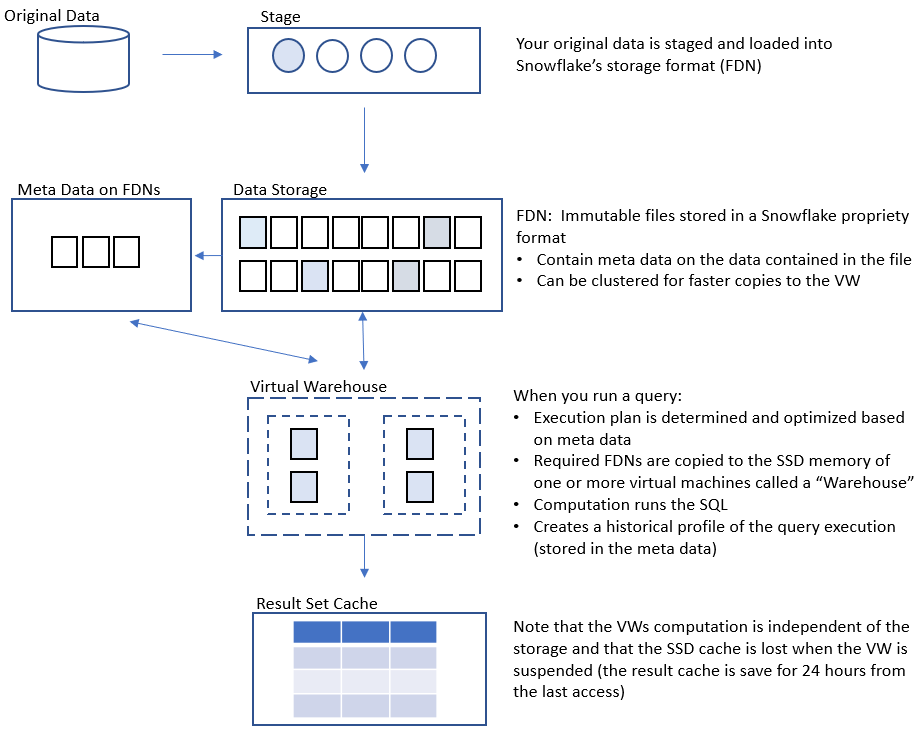
\includegraphics[width=\linewidth]{snowflake_basics.png}

\cheatsheetsubsection{Data loading}
Although very different than storing data on traditional disk, there are many benefits to loading Snowflake data strategically.
\be{}
      \item Sort on ingestion: Data is automatically partitioned in Snowflake on natural ingestion order. Sorting an S3 bucket (using something like syncsort) before bulk load via copy could be way faster than inserting with an \texttt{ORDER BY}
      \item CSV (gzipped) is the best format for loading to Snowflake (2-3x faster than Parquet or ORC)
      \item Use  instead of \texttt{INSERT} because it utilizes the more efficient bulk loading processes.
\ee{}

\cheatsheetsubsection{Sizing}

Take advantage of the native cloud ability to scale, create, and optimize your compute resources.

\be{}
      \item Scale up or out appropriately. As seen above, when you run a query, Snowflake will:
      \bi{}
            \item Find required FDN files
            \item Pull files down into SSD VMs (Note: if \> 160 GB for AWS or \> 400 GB for Azure, will \textbf{spill over} to remote IO)
            \item Performs compute
            \item Files will stay on VM \textbf{until DW is suspended}
            \item Keep in mind: 1 big query = increase size of Data Warehouse
            \item VLots of small queries = queries are queuing = increase number of DWs or increase of clusters (if enterprise you can enable multi-cluster)
      \ei{}
      \item Turn your VW on and off for certain workloads
      \bi{}
            \item Turn on for batch, then immediately turn off (no reason to wait for \textit{auto-suspend})
            \item Use \textit{auto-resume} when it makes sense
      \ei{}
      \item Control query processing and concurrency  with \href{https://docs.snowflake.net/manuals/sql-reference/parameters.html}{parameters}
      \bi{}
            \item \texttt{max\_concurrency\_level}
            \item Statement queued timeout in seconds
            \item Statement timeout in seconds
      \ei{}
      \item Use warehouse monitoring to size and limit cost per workload (not per database \ding{239} this is a shift from the on-prem mentality)
      \bi{}
            \item If your workload is queuing then add more clusters
            \item If your workload is slow with no queuing then size up...
      \ei{}

\ee{}

\cheatsheetsubsection{Data modeling}

Often overlooked, organizing your information into a mature data model will allow for high-performance SQL scripting better caching potential. Shameless plug, this is Aptitive's bread and butter. Please reach out for a free working session to discuss data modeling for your company.

\be{}
      \item Do a data model for analytics
      \item Bake your constraints into design because Snowflake \textbf{does not} enforce them
      \bi{}
            \item Build queries to check for violations
      \ei{}
      \item Build a process to alert you about loading issues
      \bi{}
            \item \texttt{information\_schema.load\_history}
            \item \href{https://aptitive.com/services/data-management/data-integration-strategy/}{Aptitive ETL Toolkit}
      \ei{}
\ee{}

\cheatsheetsubsection{Tracking Usage}

Snowflake preserves a massive amount of usage data for analysis. At the very least, it allows you to see which workflows are the most expensive.

\be{}
      \item Use Account Usage Views (eg. \texttt{warehouse\_metering\_history}) for tracking history, performance and cost
      \item Don't use \texttt{AccountAdmin} or \texttt{Public} roles for creating objects or accessing data (only for looking at costs), create securable objects with the \textit{correct} role and integrate new roles into the existing hierarchy
      \bi{}
            \item Create roles by business functions to track spending by the line of business
      \ei{}
      \item Use Resource Monitors to cut off DWs when you hit predefined credit amount limits
      \bi{}
            \item Create one resource monitor per DW
            \item Enable notifications
      \ei{}
\ee{}

\cheatsheetsubsection{Performance Tuning}

The history profiler is the primary tool to observe poorly written queries and make the appropriate changes.

\be{}
      \item Use history profiler to optimize queries
      \bi{}
            \item The goal is to put the most expensive node in the bottom right hand corner of profiler diagram
            \item \texttt{system\$clustering\_depth} shows how effective the partitions are - the smaller the average depth, the better clustered the table is with regards to the specified columns
      \ei{}
      \item Analyze Bytes Scanned: \textit{Remote} VS \textit{Cache}
      \bi{}
            \item Make your Bytes Scanned column use \textit{Cache} or \textit{Local} memory most of the time, otherwise consider creating a cluster key to scan more efficiently
      \ei{}
      \item Make the ratio of partitions scanned to partition used as small as possible by pruning
\ee{}

\cheatsheetsubsection{SQL coding}

The number one issue driving costs in a Snowflake deployment is poorly written code! Resist the tendency to just increase the power (and therefore the cost) and focus some time on improving your SQL scripts.

\be{}
      \item Drop temporary and transient tables when done using
      \item Don't use \texttt{CREATE TABLE AS}, Snowflake hates truncates and reloads for time travel issues. Instead, use \texttt{CREATE OR REPLACE}
      \bi{}
            \item Use \texttt{COPY INTO} not \texttt{INSERT INTO}
            \item Use staging tables to manage transformation of imported data
            \item Validate the data \textbf{before} loading into Snowflake target tables
      \ei{}
      \item Use ANSI joins because they are better for the optimizer
      \bi{}
            \item Use \texttt{JOIN ON a.id \= b.id} format, \textbf{NOT} the \texttt{WHERE a.id=b.id}
      \ei{}
      \item Use \texttt{WITH} clauses for windowing instead of temp tables or sub-selects
      \item Avoid using \texttt{ORDER BY}. Sorting is very expensive!
      \bi{}
      \item Use integers over strings if you must order
      \ei{}
      \item Don't handle duplicate data using \texttt{DISTINCT} or \texttt{GROUP BY}
\ee{}

\cheatsheetsubsection{Storing data}

Finally, set up the Snowflake deployment to work well in your entire data ecosystem.

\be{}
      \item Locate your S3 buckets in the same geographic region as your Snowflake instance
      \item Set up the buckets to match how the files are coming across (eg.by date or application)
      \item Keep files between 60-100 MB to take advantage of parallelism
      \item Don't use materialized views except in specific use cases (eg.pre-aggregating)
\ee{}

\cheatsheetsection{Glossary}

\be{}
      \item \href{https://docs.snowflake.com/en/sql-reference/sql/create-clone.html}{clone} \ding{239} a clone is a copy of a storage object (database / schema / table). This is typically a zero-copy clone, meaning the underlying data exists only once but metadata creates 2 different entities on top of the base data.

      \item \href{https://docs.snowflake.net/manuals/user-guide/credits.html}{credits} \ding{239} compute credits are the unit of compute in Snowflake. One credit is charged for one node running for one hour in Snowflake. Larger warehouses consist of more nodes and therefore charge more credits per hour.
      
      \item \href{https://docs.snowflake.net/manuals/user-guide/data-sharing-intro.html}{data sharing} \ding{239} secure data sharing is a unique feature of Snowflake that allows account-to-account sharing of data. This allows producers to securely expose storage objects (databases / schemas / tables) to consumers. The sharing is live and has a wide range of configurations to ensure the desired billing of storage and compute.
      
      \item \href{https://docs.snowflake.net/manuals/sql-reference/ddl-database.html}{database} \ding{239} is the top-level storage object in Snowflake. All storage objects are contained within a database. This is the highest level of data organization available.
      
      \item \href{https://docs.snowflake.net/manuals/sql-reference/sql/create-file-format.html}{file format} \ding{239} named file format is a collection of rules for processing file data to and from Snowflake stages. File format rules include data formatting, extension-specific options (like skipping headers in CSV files), and error tolerance options (like skipping files with too many errors).
      
      \item \href{https://docs.snowflake.net/manuals/user-guide/views-materialized.html}{materialized view} \ding{239} a materialized view is a stored query against 1 underlying table (this restriction may change in the future) that automatically runs behind the scenes. The query results are stored (materialized), which can improve read latency.
      
      \item \href{https://docs.snowflake.net/manuals/user-guide/security-access-control-overview.html#privileges}{privilege} \ding{239} privileges are definitions of specific access permissions to specific objects. In Snowflake's security model, privileges on objects are granted to roles. Roles are granted either to users or other roles. Privileges are never directly assigned to users.
      
      \item \href{https://docs.snowflake.net/manuals/user-guide/security-access-control-overview.html#roles}{role} \ding{239} a role is the unit of Snowflake security to which privileges can be granted to or revoked from. Roles are not users but are assigned to users to authorize user activity.
      
      \item \href{https://docs.snowflake.net/manuals/sql-reference/ddl-database.html#schema-management}{schema} \ding{239} a schema is the second layer of storage organization in Snowflake below a database. They are containers that hold tables, views, stages, and other bottom-level objects. Security objects and warehouses are not stored at this level. A schema and a database together define a namespace in Snowflake.
      
      \item \href{https://docs.snowflake.net/manuals/user-guide/querying-sequences.html}{sequence} \ding{239} a sequence is a generator object that creates unique values in SQL statements that cover many rows. This is an advanced SQL concept. \href{https://www.geeksforgeeks.org/sql-sequences/}{Check out this article that gives an overview of the concept.}
      
      \item \href{https://docs.snowflake.net/manuals/user-guide/data-load-snowpipe-intro.html}{Snowpipe} \ding{239} this refers to Snowflake's continuous loading solution. It is confusing right now because Snowpipe is being upgraded for asynchronous file handling through queues, but not all instances will have this ability (auto ingest). In short, all Snowpipes make regular file ingestion from external stages more manageable for your production workflows.
      
      \item \href{https://docs.snowflake.net/manuals/user-guide/snowsql.html}{SnowSQL} \ding{239} SnowSQL refers to the Snowflake CLI tool. It's also commonly used to refer to the actual SQL code that is run in Snowflake.
      
      \item \href{https://docs.snowflake.net/manuals/sql-reference/sql/create-stage.html}{stage} \ding{239} this is a file location used for data ingestion. Stages can either be internal (managed by Snowflake) or external (managed by you). Stages are just S3 (AWS) or Blob Storage Containers (Azure) where data in Snowflake-supported file formats can be stored before loading into a Snowflake table. Understanding stages is critical to building production data pipelines.
      
      \item \href{https://docs.snowflake.net/manuals/sql-reference/stored-procedures-overview.html}{stored procedures} \ding{239} stored procedures are reusable functions defined with a mix of JavaScript and SQL for advanced functionality. These are useful for implementing logic with \href{https://developer.mozilla.org/en-US/docs/Glossary/Control_flow}{advanced control flow} requirements that are unsupported by SQL (error handling, for-loops, conditional branching).
      
      \item \href{https://docs.snowflake.net/manuals/user-guide/streams.html}{streams} \ding{239} streams are change records on top of tables. They are queryable like normal tables but include an automatically-updated record of every data change that occurred on the target object. These are a preview feature, so make sure you have it enabled.
      
      \item \href{https://docs.snowflake.net/manuals/sql-reference/ddl-table.html}{table} \ding{239} a table is the lowest level object in Snowflake. It is a structured collection of persisted data.
      
      \item \href{https://docs.snowflake.net/manuals/user-guide/tasks.html}{tasks} \ding{239} a task is a SQL statement executed either on a schedule or in response to the completion of another task. Tasks are useful for job scheduling and are currently preview features.
      
      \item \href{https://docs.snowflake.net/manuals/user-guide/tables-temp-transient.html#temporary-tables}{temporary table} \ding{239} these tables exist only for the duration of a session and are not queriable by any other user. This is useful for ETL processing and helps reduce storage costs as temp tables do not use the same amount of failsafe storage that a standard table does.
      
      \item \href{https://docs.snowflake.net/manuals/user-guide/data-time-travel.html}{time travel} \ding{239} this feature enables users to query data at different points within a range of time (configured at the storage object level). The longer the range of time (up to 90 days, but 1 day by default), the more storage charges are incurred. This feature is valuable for comparing state over time without having to manage additional complex storage structures.
      
      \item \href{https://docs.snowflake.net/manuals/sql-reference/transactions.html}{transaction} \ding{239} transaction is a collection of SQL statements that must either be entirely executed successfully or entirely unexecuted (no partial execution). These transactions are fully \href{https://en.wikipedia.org/wiki/ACID}{ACID compliant}.
      
      \item \href{https://docs.snowflake.net/manuals/user-guide/tables-temp-transient.html#transient-tables}{transient table} \ding{239} transient tables are really similar to temporary tables, but they persist beyond a single session and can be queried by other users. They differ from standard tables by having no failsafe storage, making them cheaper but less durable.
      
      \item \href{https://docs.snowflake.net/manuals/sql-reference/udf-overview.html}{User defined function (UDF)} \ding{239} a UDF is a named collection of either SQL or JavaScript logic that accepts arguments and returns either a scalar (single value) or series of rows, depending on how it is defined. It does not support the creation or modification of objects (DML) and only returns newly computed values.
      
      \item \href{https://docs.snowflake.net/manuals/user-guide/admin-user-management.html}{user} \ding{239} a user is an entity of authentication. Authorization is granted to users through roles. Roles are a named collection of 0 or more privileges to perform actions with Snowflake objects. Users are often associated with individuals but are also used to authenticate services, such as BI connections.
      
      \item \href{https://docs.snowflake.net/manuals/user-guide/views-introduction.html}{view} \ding{239} a view is a table-like object that can be queried but stores no actual data. The structure of a view is defined when it is created as a SQL statement that selects from other underlying objects (including other views).
      
      \item \href{https://docs.snowflake.net/manuals/user-guide/warehouses-overview.html}{warehouse} \ding{239} a virtual warehouse is the object of compute in Snowflake. The size of a warehouse indicates how many nodes are in the compute cluster used to run queries. Warehouses are needed to load data from cloud storage and perform computations. They retain source data in a node-level cache as long as they are not suspended. Snowflake credits are billed for a 1-node (XSMALL) warehouse running for 1 hour (10-second minimum charge, prorated per second of run after that).
      
      \item \href{https://docs.snowflake.net/manuals/user-guide/ui-worksheet.html}{worksheet} \ding{239} worksheet is a tab within the Snowflake Web UI with its own distinct context from the user's logged-in context. Each worksheet has a SQL editor space where SQL is commonly developed and ran in one location.
\ee{}
The glossary was taken from \href{https://community.snowflake.com/s/article/30-Second-Snowflake-Cloud-Data-Warehouse-Cheat-Sheet}{this} page.

\vfill

\cheatsheetfooter{Created by Piotr Szwajkowski}{mail@piotrszwajkowski.com}

\end{multicols}

\end{document}
